\documentclass[preview]{standalone}

\usepackage{amsmath}
\usepackage{amssymb}
\usepackage{tikz}
\usepackage{stellar}
\usepackage{bettelini}

\hypersetup{
    colorlinks=true,
    linkcolor=black,
    urlcolor=blue,
    pdftitle={Assets},
    pdfpagemode=FullScreen,
}

\begin{document}

\title{Sfere Terrestri}
\id{geofisica-sfereterrestri}
\genpage

\section{Sfere terrestri}

\plain{La terra può essere suddivisa in diverse sfere interdipendenti.}

\begin{snippetdefinition}{atmosfera-definition}{Atmosfera}
    Componente gassosa che avvolge il pianeta. L'aria è inodore e incolore ed è quasi 800 volte meno densa dell'acqua.
\end{snippetdefinition}

\begin{snippetdefinition}{idrosfera-definition}{Idrosfera}
    Insieme di tutte le acque del pianeta nei diversi stati di aggregazione; comprende le acque marine e quelle continentali.
\end{snippetdefinition}
    
\begin{snippetdefinition}{litosfera-definition}{Litosfera}
    Componente solida superficiale costituita dalle rocce.
\end{snippetdefinition}

\begin{snippetdefinition}{biosfera-definition}{Biosfera}
    Componente vivente e comprende gli organismi che popolano la zona di interazione dell'atmosfera, idrosfera e litosfera.
\end{snippetdefinition}

\begin{snippetdefinition}{astenosfera-definition}{Astenosfera}
    L'\textit{astenosfera} è una fascia superficiale del mantello terrestre, giacente sotto la litosfera,
    dove le roccie sono parzialmente fuse.
\end{snippetdefinition}

\begin{snippetdefinition}{processo-esogeno}{Processo Esogeno}
    Sono processi attivati dall'energia del Sole e avvengono sulla superficie terrestre; sono per esempio i movimento delle acque, i passaggi di stato, il tempo atmosferi o il modellamento della superficie terrestre.
\end{snippetdefinition}

\begin{snippetdefinition}{processo-endogeno}{Processo Endogeno}
    Sono processi attivati dal calore interno della Terra; sono i processi che portano alla formazione di catene montuose e di nuovi oceani.
\end{snippetdefinition}

\plain{I processi che coinvologno le sfere terrestri sono di tipo esogeno ed endogeno.
I processi esogeni possono includere alterazione meteorica, movimenti di massa, erosione,
mentre i processi endogeni vulcanismo, riorganizzazione crostale e diastrofismo.}

\section{Il geosistema tettonica delle placche}

\begin{snippet}{earth-cutaway-schematic-it}
    \begin{figure*}[h]
        \begin{center}
            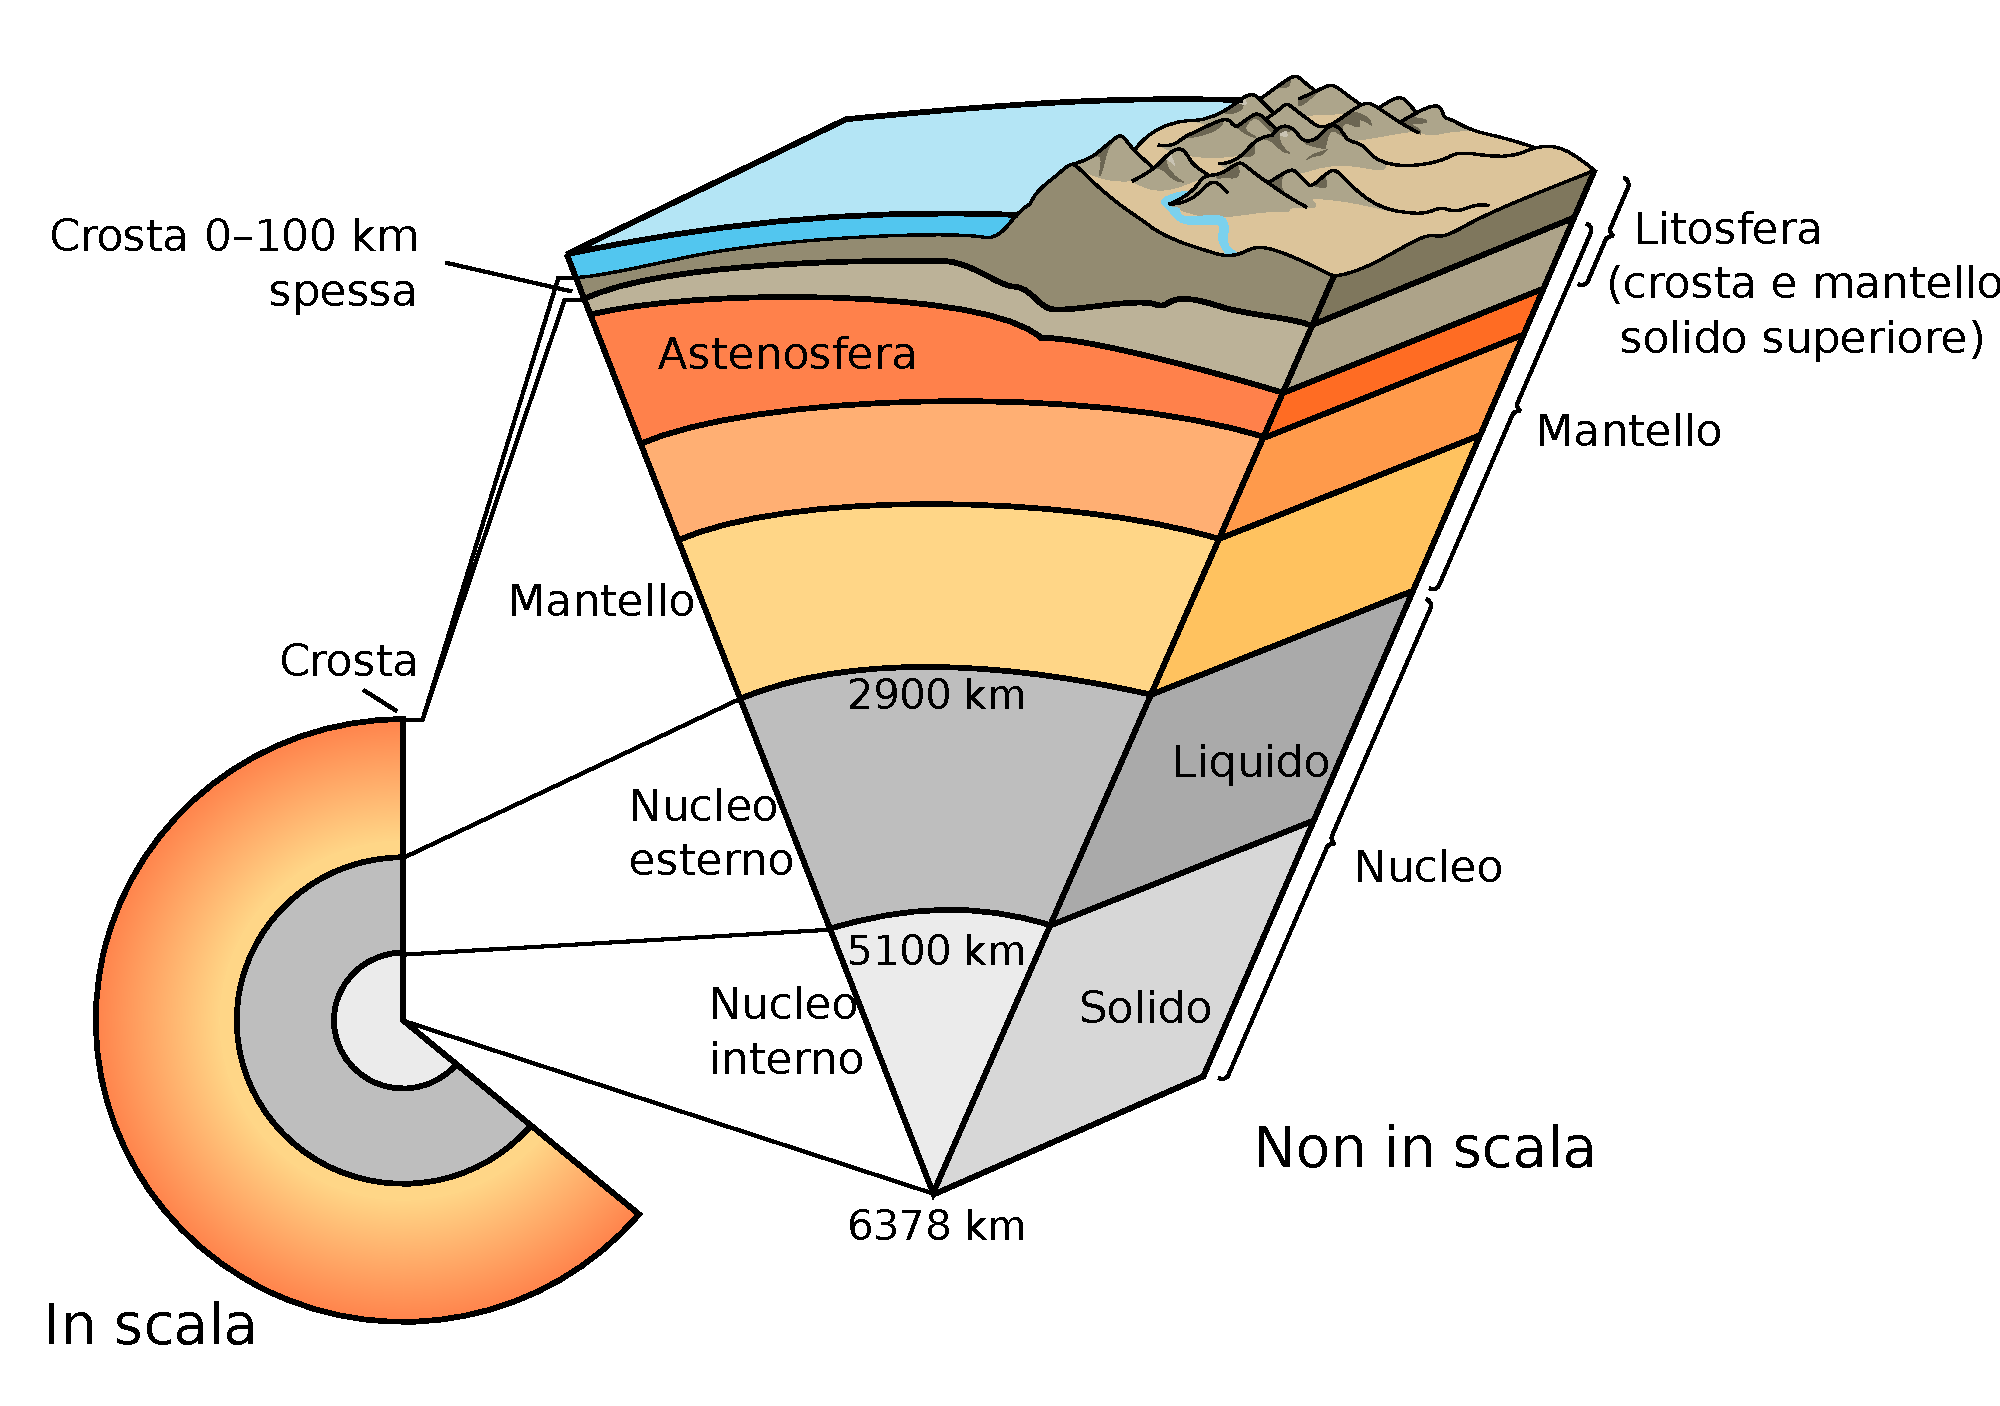
\includegraphics[width=.8\textwidth]{resources/earth-cutaway-schematic-it.pdf}
        \end{center}
    \end{figure*}
\end{snippet}

\end{document}